%%%%%%%%%%%%%%%%%%%%%%%%%%%%%%%%%%%%%%%%%%%%%%%%

% Specify the command that you want into the header of the
% index.md file

%%%%%%%%%%%%%%%%%%%%%%%%%%%%%%%%%%%%%%%%%%%%%%%%

% Options for packages loaded elsewhere
\PassOptionsToPackage{unicode}{hyperref}
\PassOptionsToPackage{hyphens}{url}
\PassOptionsToPackage{dvipsnames,svgnames*,x11names*}{xcolor}
%
\documentclass[
  12pt,
  oneside]{report}
%%\usepackage{lmodern}
%
% Set line spacing
\usepackage{setspace}
\setstretch{1.5}

\usepackage{amssymb,amsmath}
\usepackage{ifxetex,ifluatex}
\ifnum 0\ifxetex 1\fi\ifluatex 1\fi=0 % if pdftex
  \usepackage[T1]{fontenc}
  \usepackage[utf8]{inputenc}
  \usepackage{textcomp} % provide euro and other symbols
\else % if luatex or xetex
  \usepackage{unicode-math}
  \defaultfontfeatures{Scale=MatchLowercase}
  \defaultfontfeatures[\rmfamily]{Ligatures=TeX,Scale=1}
\fi
% Use upquote if available, for straight quotes in verbatim environments
\IfFileExists{upquote.sty}{\usepackage{upquote}}{}
\IfFileExists{microtype.sty}{% use microtype if available
  \usepackage[]{microtype}
  \UseMicrotypeSet[protrusion]{basicmath} % disable protrusion for tt fonts
}{}
\makeatletter
\@ifundefined{KOMAClassName}{% if non-KOMA class
  \IfFileExists{parskip.sty}{%
    \usepackage{parskip}
  }{% else
    \setlength{\parindent}{0pt}
    \setlength{\parskip}{6pt plus 2pt minus 1pt}}
}{% if KOMA class
  \KOMAoptions{parskip=half}}
\makeatother
\usepackage{xcolor}
\IfFileExists{xurl.sty}{\usepackage{xurl}}{} % add URL line breaks if available
\IfFileExists{bookmark.sty}{\usepackage{bookmark}}{\usepackage{hyperref}}
\hypersetup{
  pdfauthor={François Leroy, PhD student at CZU},
  colorlinks=true,
  linkcolor=Maroon,
  filecolor=Maroon,
  citecolor=Blue,
  urlcolor=Blue,
  pdfcreator={LaTeX via pandoc}}
\urlstyle{same} % disable monospaced font for URLs

%% Package geometry
\usepackage[left = 2cm,right = 2cm,top = 2cm,bottom = 2cm]{geometry}
\usepackage{pdflscape}


\usepackage{color}
\usepackage{fancyvrb}
\newcommand{\VerbBar}{|}
\newcommand{\VERB}{\Verb[commandchars=\\\{\}]}
\DefineVerbatimEnvironment{Highlighting}{Verbatim}{commandchars=\\\{\}}
% Add ',fontsize=\small' for more characters per line
\usepackage{framed}
\definecolor{shadecolor}{RGB}{248,248,248}
\newenvironment{Shaded}{\begin{snugshade}}{\end{snugshade}}
\newcommand{\AlertTok}[1]{\textcolor[rgb]{0.94,0.16,0.16}{#1}}
\newcommand{\AnnotationTok}[1]{\textcolor[rgb]{0.56,0.35,0.01}{\textbf{\textit{#1}}}}
\newcommand{\AttributeTok}[1]{\textcolor[rgb]{0.77,0.63,0.00}{#1}}
\newcommand{\BaseNTok}[1]{\textcolor[rgb]{0.00,0.00,0.81}{#1}}
\newcommand{\BuiltInTok}[1]{#1}
\newcommand{\CharTok}[1]{\textcolor[rgb]{0.31,0.60,0.02}{#1}}
\newcommand{\CommentTok}[1]{\textcolor[rgb]{0.56,0.35,0.01}{\textit{#1}}}
\newcommand{\CommentVarTok}[1]{\textcolor[rgb]{0.56,0.35,0.01}{\textbf{\textit{#1}}}}
\newcommand{\ConstantTok}[1]{\textcolor[rgb]{0.00,0.00,0.00}{#1}}
\newcommand{\ControlFlowTok}[1]{\textcolor[rgb]{0.13,0.29,0.53}{\textbf{#1}}}
\newcommand{\DataTypeTok}[1]{\textcolor[rgb]{0.13,0.29,0.53}{#1}}
\newcommand{\DecValTok}[1]{\textcolor[rgb]{0.00,0.00,0.81}{#1}}
\newcommand{\DocumentationTok}[1]{\textcolor[rgb]{0.56,0.35,0.01}{\textbf{\textit{#1}}}}
\newcommand{\ErrorTok}[1]{\textcolor[rgb]{0.64,0.00,0.00}{\textbf{#1}}}
\newcommand{\ExtensionTok}[1]{#1}
\newcommand{\FloatTok}[1]{\textcolor[rgb]{0.00,0.00,0.81}{#1}}
\newcommand{\FunctionTok}[1]{\textcolor[rgb]{0.00,0.00,0.00}{#1}}
\newcommand{\ImportTok}[1]{#1}
\newcommand{\InformationTok}[1]{\textcolor[rgb]{0.56,0.35,0.01}{\textbf{\textit{#1}}}}
\newcommand{\KeywordTok}[1]{\textcolor[rgb]{0.13,0.29,0.53}{\textbf{#1}}}
\newcommand{\NormalTok}[1]{#1}
\newcommand{\OperatorTok}[1]{\textcolor[rgb]{0.81,0.36,0.00}{\textbf{#1}}}
\newcommand{\OtherTok}[1]{\textcolor[rgb]{0.56,0.35,0.01}{#1}}
\newcommand{\PreprocessorTok}[1]{\textcolor[rgb]{0.56,0.35,0.01}{\textit{#1}}}
\newcommand{\RegionMarkerTok}[1]{#1}
\newcommand{\SpecialCharTok}[1]{\textcolor[rgb]{0.00,0.00,0.00}{#1}}
\newcommand{\SpecialStringTok}[1]{\textcolor[rgb]{0.31,0.60,0.02}{#1}}
\newcommand{\StringTok}[1]{\textcolor[rgb]{0.31,0.60,0.02}{#1}}
\newcommand{\VariableTok}[1]{\textcolor[rgb]{0.00,0.00,0.00}{#1}}
\newcommand{\VerbatimStringTok}[1]{\textcolor[rgb]{0.31,0.60,0.02}{#1}}
\newcommand{\WarningTok}[1]{\textcolor[rgb]{0.56,0.35,0.01}{\textbf{\textit{#1}}}}
\usepackage{longtable,booktabs}
% Correct order of tables after \paragraph or \subparagraph
\usepackage{etoolbox}
\makeatletter
\patchcmd\longtable{\par}{\if@noskipsec\mbox{}\fi\par}{}{}
\makeatother
% Allow footnotes in longtable head/foot
\IfFileExists{footnotehyper.sty}{\usepackage{footnotehyper}}{\usepackage{footnote}}
\makesavenoteenv{longtable}
\usepackage{graphicx}
\makeatletter
\def\maxwidth{\ifdim\Gin@nat@width>\linewidth\linewidth\else\Gin@nat@width\fi}
\def\maxheight{\ifdim\Gin@nat@height>\textheight\textheight\else\Gin@nat@height\fi}
\makeatother
% Scale images if necessary, so that they will not overflow the page
% margins by default, and it is still possible to overwrite the defaults
% using explicit options in \includegraphics[width, height, ...]{}
\setkeys{Gin}{width=\maxwidth,height=\maxheight,keepaspectratio}
% Set default figure placement to htbp
\makeatletter
\def\fps@figure{htbp}
\makeatother
\setlength{\emergencystretch}{3em} % prevent overfull lines
\providecommand{\tightlist}{%
  \setlength{\itemsep}{0pt}\setlength{\parskip}{0pt}}
\setcounter{secnumdepth}{5}
%%% Complete the preamble of the LaTeX template
%%%------------------------------------------------------------------------------

%% Bug de bookdown: ne traite plus la déclaration "otherlangs" dans le préambule
% Pour charger les langues, écriture ici en dur du produit de bookdown
% Corrigé le 22/11/2019. A retester régulièrement: supprimer ces lignes si la compilation fonctionne sans elles.
\usepackage{polyglossia}
  \setmainlanguage[variant=american]{english}
  \setotherlanguage[]{french}
% Bug persistant le 28/02/2020

% Advised with polyglossia and babel
\usepackage{csquotes}

% Environnement "Essentiel" en début de chapitre
\usepackage[tikz]{bclogo}
\newenvironment{Essentiel}
  {\begin{bclogo}[logo=\bctrombone, noborder=true, couleur=lightgray!50]{L'essentiel}\parindent0pt}
  {\end{bclogo}}

%% Package fontspec
\usepackage{fontspec}
\setmainfont{calibri}[
  Path           = ./fonts/,
  Extension      = .ttf,
  BoldFont       = calibrib,
  ItalicFont     = calibrili,
  BoldItalicFont = calibriz]

% Rename chapters
% Below, scrpit to prevent the "chapter n" and the space use for it to
% be displayed
\usepackage{titlesec}
\titleformat{\chapter}   
{\Huge}{\thechapter{. }}{0pt}{\Huge}
%{\thechapter{. }}
\titlespacing*{\chapter}{0pt}{-50pt}{10pt}
% -50 is to up the title and 10 is the space with the text below
\usepackage{booktabs}
\usepackage{longtable}
\usepackage{array}
\usepackage{multirow}
\usepackage{wrapfig}
\usepackage{float}
\usepackage{colortbl}
\usepackage{pdflscape}
\usepackage{tabu}
\usepackage{threeparttable}
\usepackage{threeparttablex}
\usepackage[normalem]{ulem}
\usepackage{makecell}
\usepackage{xcolor}
\ifluatex
  \usepackage{selnolig}  % disable illegal ligatures
\fi

\title{Introduction to Machine Learning\\
(NPFL054)}
\usepackage{etoolbox}
\makeatletter
\providecommand{\subtitle}[1]{% add subtitle to \maketitle
  \apptocmd{\@title}{\par {\large #1 \par}}{}{}
}
\makeatother
\subtitle{Homework 2}
\author{François Leroy, PhD student at CZU}
\date{2021-06-01}

% to include pdf
\usepackage{pdfpages}



%%%%%%%%%%%%%%%%%%%%%%%%%%%%%%%%%%%%%%%%%%%%%%%%%%%%%%%%%%%%%
% Start of the documents
\begin{document}
\maketitle


% Roman numbering for content before toc and toc itself
\cleardoublepage 
\pagenumbering{roman}

{
\hypersetup{linkcolor=}
\setcounter{tocdepth}{1}
\tableofcontents
\newpage
}
\vspace{50mm}
\setstretch{1.5}


% Start the arabic numbering at the 1st chapter
\cleardoublepage 
\pagenumbering{arabic}


% The mind, the...
\hypertarget{set-up-the-project}{%
\chapter*{Set up the project}\label{set-up-the-project}}
\addcontentsline{toc}{chapter}{Set up the project}

\begin{Shaded}
\begin{Highlighting}[]
\KeywordTok{rm}\NormalTok{(}\DataTypeTok{list =} \KeywordTok{ls}\NormalTok{())}
\KeywordTok{library}\NormalTok{(ISLR) }\CommentTok{# for the data}
\KeywordTok{library}\NormalTok{(tidyverse) }\CommentTok{# convenient}
\KeywordTok{library}\NormalTok{(rpart) }\CommentTok{# for decision trees}
\KeywordTok{library}\NormalTok{(randomForest) }\CommentTok{# for ensemble learning}
\KeywordTok{library}\NormalTok{(glmnet) }\CommentTok{# for regularized logistic regression}
\KeywordTok{library}\NormalTok{(ROCR) }\CommentTok{# for ROC curves}
\end{Highlighting}
\end{Shaded}

\begin{Shaded}
\begin{Highlighting}[]
\CommentTok{## Reproduce the result}
\KeywordTok{set.seed}\NormalTok{(}\DecValTok{123}\NormalTok{)}
\CommentTok{## Create the splitting vector}
\NormalTok{split <-}\StringTok{ }\KeywordTok{sample}\NormalTok{(}\KeywordTok{nrow}\NormalTok{(Caravan), }\DecValTok{1000}\NormalTok{)}
\CommentTok{## Create the test dataset}
\NormalTok{d_test <-}\StringTok{ }\NormalTok{Caravan[split,]}
\CommentTok{## Create the training dataset}
\NormalTok{d_train <-}\StringTok{ }\NormalTok{Caravan[}\OperatorTok{-}\NormalTok{split,]}
\end{Highlighting}
\end{Shaded}

\hypertarget{task1}{%
\chapter{Task 1 - Data analysis}\label{task1}}

\begin{itemize}
\tightlist
\item
  \textbf{First, check the distribution of the target attribute. What would be your precision if you select 100 examples by chance?}
\end{itemize}

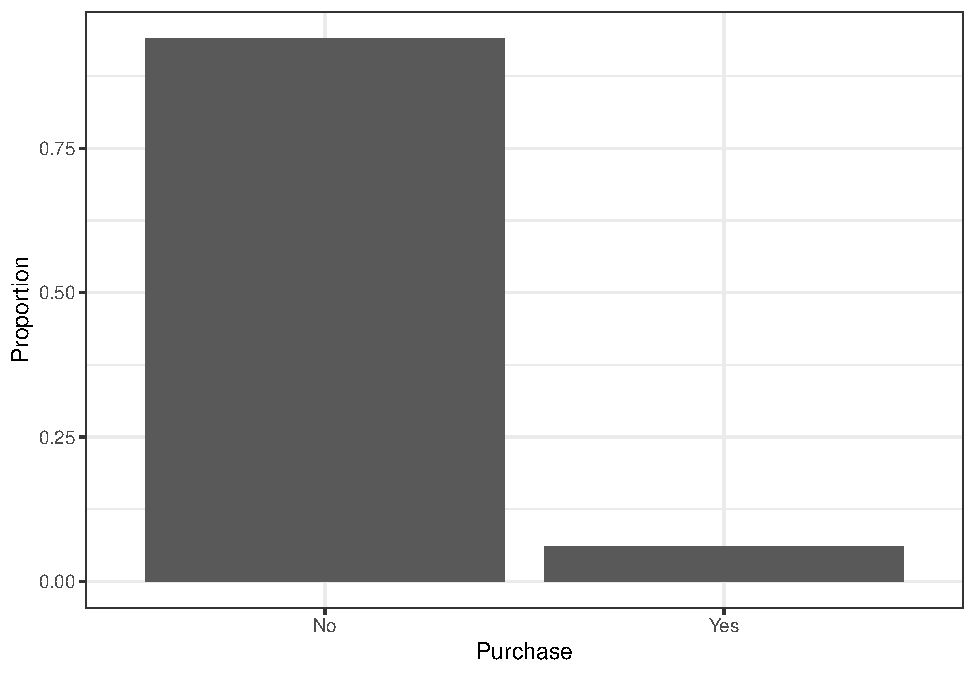
\includegraphics{leroy_francois_hw2_files/figure-latex/unnamed-chunk-5-1.pdf}

We can see that there is 94\% of customers who didn't purchase the insurance and that 6\% who did. From this, we can compute the following Probability Mass Function of this binomial distribution:

\begin{Shaded}
\begin{Highlighting}[]
\KeywordTok{plot}\NormalTok{(}\KeywordTok{dbinom}\NormalTok{(}\DecValTok{1}\OperatorTok{:}\DecValTok{20}\NormalTok{, }\DataTypeTok{size =} \DecValTok{100}\NormalTok{, }\DataTypeTok{prob =} \FloatTok{.06}\NormalTok{))}
\end{Highlighting}
\end{Shaded}

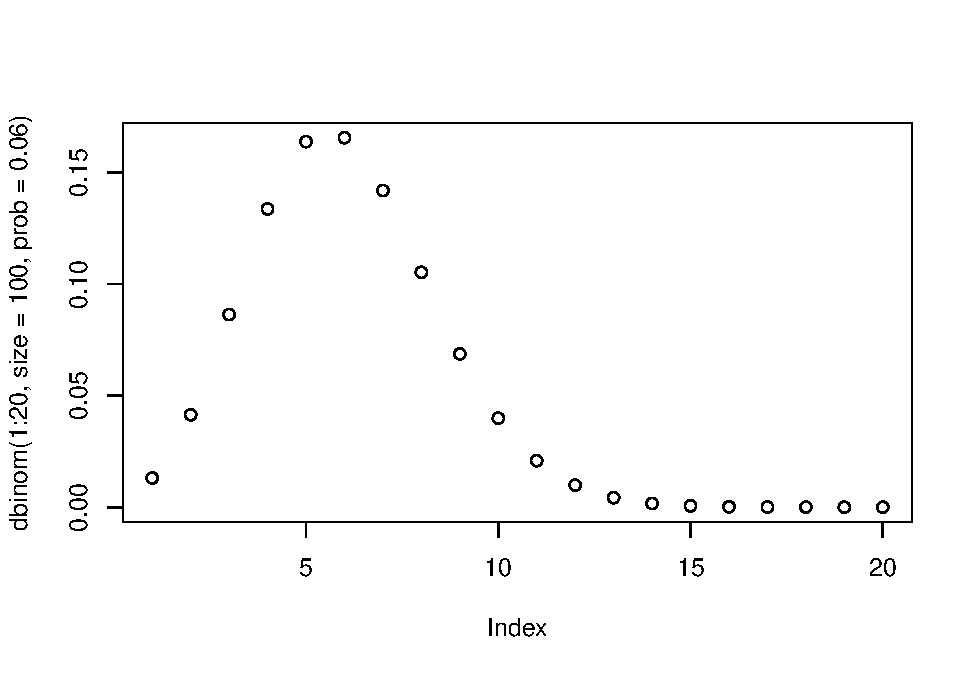
\includegraphics{leroy_francois_hw2_files/figure-latex/unnamed-chunk-6-1.pdf}

The precision is the number of examples classified as \emph{Yes} when the value is actually \emph{Yes}. Here, the precision should be 0.06, which is actually the ratio between \enquote{Yes} and \enquote{No}.

\begin{itemize}
\tightlist
\item
  \textbf{1.a. Focus on the customer type MOSHOOFD: create a table with the number of customers that belong to each of 10 L2 groups and the percentage of customers that purchased a caravan insurance policy in each group. Comment the figures in the table. Then do the same for the customer subtype MOSTYPE (41 subgroups defined in L1).}
\end{itemize}

\underline{MOSHOOFD type:}

\begin{Shaded}
\begin{Highlighting}[]
\NormalTok{Caravan }\OperatorTok\StringTok{ }
\StringTok{  }\KeywordTok{count}\NormalTok{(MOSHOOFD, Purchase) }\OperatorTok\StringTok{ }
\StringTok{  }\KeywordTok{group_by}\NormalTok{(MOSHOOFD) }\OperatorTok\StringTok{ }
\StringTok{  }\KeywordTok{summarise}\NormalTok{(}\DataTypeTok{size =} \KeywordTok{sum}\NormalTok{(n),}
            \DataTypeTok{purchase_prop =} \KeywordTok{round}\NormalTok{(n[Purchase }\OperatorTok{==}\StringTok{ "Yes"}\NormalTok{]}\OperatorTok{/}\KeywordTok{sum}\NormalTok{(n), }\DecValTok{2}\NormalTok{)) }\OperatorTok\StringTok{ }
\StringTok{  }\KeywordTok{rename}\NormalTok{(}\DataTypeTok{group =}\NormalTok{ MOSHOOFD) }\OperatorTok\StringTok{ }
\StringTok{  }\NormalTok{kableExtra}\OperatorTok{::}\KeywordTok{kable}\NormalTok{()}
\end{Highlighting}
\end{Shaded}

\begin{tabular}{r|r|r}
\hline
group & size & purchase\_prop\\
\hline
1 & 552 & 0.09\\
\hline
2 & 502 & 0.13\\
\hline
3 & 886 & 0.07\\
\hline
5 & 569 & 0.03\\
\hline
6 & 205 & 0.02\\
\hline
7 & 550 & 0.04\\
\hline
8 & 1563 & 0.06\\
\hline
9 & 667 & 0.06\\
\hline
10 & 276 & 0.02\\
\hline
\end{tabular}

This table shows the number of individuals (column \(size\)) and the proportion of customers that will buy an insurance in each group (column \(purchase\_prop\)) of the \emph{MOSHOOFD} variable. The \emph{MOSHOOFD} attribute correspond to the customer main type. We can see that the customers that are more prone to purchase an insurance are the one belonging to the group 2, \emph{i.e.} the \emph{driven growers} (13\% of them will buy an insurance). Then, the \emph{successful hedonist} are more likely to buy an insurance (\emph{group 1}, \(9\%\) of them). The names of these two groups suggest that they are rather wealthy individuals. On the other hand, the customers belonging to the class 6 and 10, respectively the \emph{cruising seniors} and the \emph{farmers}, are less likely to subscribe to the insurance (only 2\% in each group). This is also quite expected, as seniors and farmers can be in precarious situations.

\underline{MOSTYPE type:}

\begin{Shaded}
\begin{Highlighting}[]
\NormalTok{table <-}\StringTok{ }
\NormalTok{Caravan }\OperatorTok\StringTok{ }
\StringTok{  }\KeywordTok{count}\NormalTok{(MOSTYPE, Purchase) }\OperatorTok\StringTok{ }
\StringTok{  }\KeywordTok{group_by}\NormalTok{(MOSTYPE) }\OperatorTok\StringTok{ }
\StringTok{  }\KeywordTok{summarise}\NormalTok{(}\DataTypeTok{size =} \KeywordTok{sum}\NormalTok{(n),}
            \DataTypeTok{purchase_prop =} \KeywordTok{round}\NormalTok{(n[Purchase }\OperatorTok{==}\StringTok{ "Yes"}\NormalTok{]}\OperatorTok{/}\KeywordTok{sum}\NormalTok{(n), }\DecValTok{2}\NormalTok{)) }\OperatorTok\StringTok{ }
\StringTok{  }\KeywordTok{rename}\NormalTok{(}\DataTypeTok{group =}\NormalTok{ MOSTYPE) }\OperatorTok\StringTok{ }
\StringTok{  }\KeywordTok{arrange}\NormalTok{(}\KeywordTok{desc}\NormalTok{(purchase_prop))}
\CommentTok{## Display in 2 columns}
\NormalTok{kableExtra}\OperatorTok{::}\KeywordTok{kable}\NormalTok{(}\KeywordTok{list}\NormalTok{(table[}\DecValTok{1}\OperatorTok{:}\NormalTok{(}\KeywordTok{nrow}\NormalTok{(table)}\OperatorTok{/}\DecValTok{2}\NormalTok{),], }
\NormalTok{                       table[((}\KeywordTok{nrow}\NormalTok{(table)}\OperatorTok{/}\DecValTok{2}\NormalTok{)}\OperatorTok{+}\DecValTok{1}\NormalTok{)}\OperatorTok{:}\KeywordTok{nrow}\NormalTok{(table),])) }\OperatorTok\StringTok{ }
\StringTok{  }\NormalTok{kableExtra}\OperatorTok{::}\KeywordTok{kable_styling}\NormalTok{(}\DataTypeTok{latex_options =} \StringTok{"HOLD_position"}\NormalTok{)}
\end{Highlighting}
\end{Shaded}

\begin{table}[H]

\centering
\begin{tabular}[t]{r|r|r}
\hline
group & size & purchase\_prop\\
\hline
8 & 339 & 0.15\\
\hline
12 & 111 & 0.14\\
\hline
1 & 124 & 0.10\\
\hline
3 & 249 & 0.10\\
\hline
6 & 119 & 0.10\\
\hline
20 & 25 & 0.08\\
\hline
37 & 132 & 0.08\\
\hline
2 & 82 & 0.07\\
\hline
7 & 44 & 0.07\\
\hline
13 & 179 & 0.07\\
\hline
36 & 225 & 0.07\\
\hline
38 & 339 & 0.07\\
\hline
11 & 153 & 0.06\\
\hline
32 & 141 & 0.06\\
\hline
33 & 810 & 0.06\\
\hline
39 & 328 & 0.06\\
\hline
\end{tabular}
\centering
\begin{tabular}[t]{r|r|r}
\hline
group & size & purchase\_prop\\
\hline
10 & 165 & 0.05\\
\hline
34 & 182 & 0.05\\
\hline
4 & 52 & 0.04\\
\hline
5 & 45 & 0.04\\
\hline
9 & 278 & 0.04\\
\hline
22 & 98 & 0.04\\
\hline
35 & 214 & 0.04\\
\hline
24 & 180 & 0.03\\
\hline
30 & 118 & 0.03\\
\hline
31 & 205 & 0.03\\
\hline
23 & 251 & 0.02\\
\hline
25 & 82 & 0.02\\
\hline
26 & 48 & 0.02\\
\hline
27 & 50 & 0.02\\
\hline
29 & 86 & 0.02\\
\hline
41 & 205 & 0.02\\
\hline
\end{tabular}
\end{table}

This table is the same than the previous one but for the \emph{MOSTYPE} variable, which gives more information about the social status. It is order by descending proportion of purchase. The two groups more prone to buy an insurance are the group 8 and 12, which correspond respectively to \emph{middle class families} and \emph{affluent young families}. Thus, we can say that families are potential good targets to sell insurances. We can see that the class 25, 26, 27 and 29 all have a low proportion of individuals buying a insurance. They are all related to old people (\emph{i.e.}, \emph{Young seniors in the city}, \emph{Own home elderly}, \emph{Seniors in apartments}, \emph{Porchless seniors: no front yard}). Thus, as said just above for the \emph{MOSHOOFD} variable, old people don't seem to be good targets to sell insurances. Moreover, the group 41, \emph{i.e.} the \emph{mixed rurals} are also less prone to subscribe an insurance, as expected with the \emph{MOSHOOFD} variable (with \emph{farmers} less prone to buy an insurance).

\textbf{1.b. Analyze the relationship between features MOSHOOFD and MOSTYPE.}

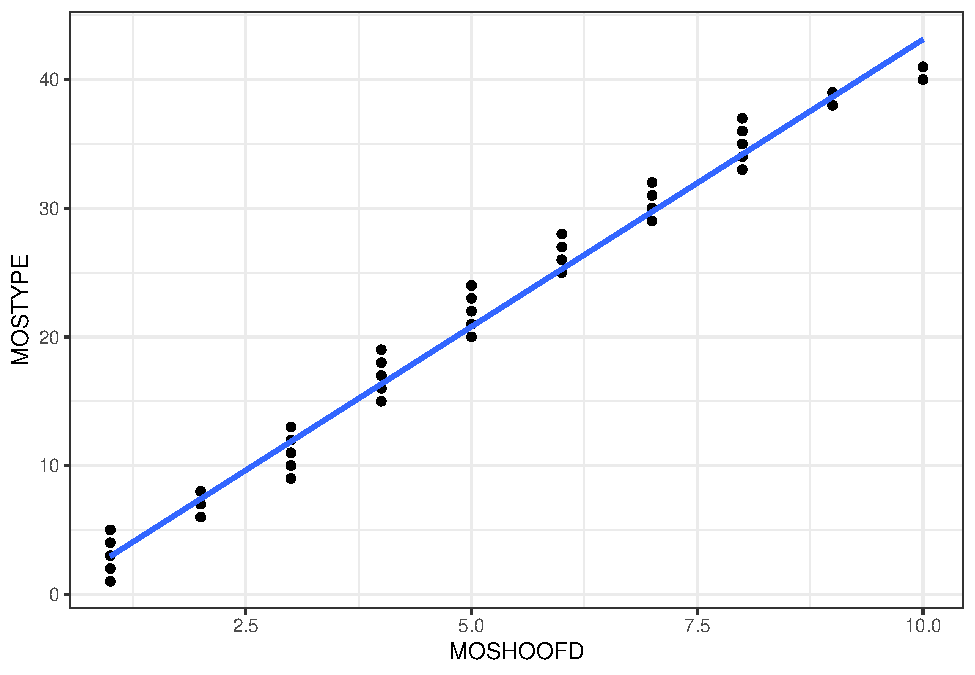
\includegraphics{leroy_francois_hw2_files/figure-latex/unnamed-chunk-9-1.pdf}

We can clearly see a relationship between these two features which are MOSHOOFD = \emph{Customer main type} and MOSTYPE = \emph{Customer Subtype}. This is expected because MOSTYPE is just a more precise social position. For instance, we can see that when \(MOSHOOFD = 10\), \(MOSTYPE = 40 | 41\). We can see that \(MOSHOOFD = 10\) correspond to \emph{Farmers} and that \(MOSTYPE = 40 | 41\) are two subclasses of farmers: \emph{Large family farms} and \emph{Mixed rurals}, respectively.

\hypertarget{task-2---model-fitting-optimization-and-selection}{%
\chapter{Task 2 - Model fitting, optimization, and selection}\label{task-2---model-fitting-optimization-and-selection}}

\begin{Shaded}
\begin{Highlighting}[]
\CommentTok{## Function to randomly extract the test dataset in d_train }
\CommentTok{## using always the same number of positive and negative }
\CommentTok{## values of Purchase}
\NormalTok{prepare_cv_folds <-}\StringTok{  }\ControlFlowTok{function}\NormalTok{(k)\{}
  \CommentTok{# Create the subsets data containing Purchase == Yes }
  \CommentTok{# in one hand and Purchase == No in an other hand}
\NormalTok{  pos_data <-}\StringTok{ }\NormalTok{d_train[d_train}\OperatorTok{$}\NormalTok{Purchase }\OperatorTok{==}\StringTok{ "Yes"}\NormalTok{,]}
\NormalTok{  neg_data <-}\StringTok{ }\NormalTok{d_train[d_train}\OperatorTok{$}\NormalTok{Purchase }\OperatorTok{==}\StringTok{ "No"}\NormalTok{,]}
  \CommentTok{## Compute the size of each fold}
\NormalTok{  fold.size.pos <-}\StringTok{ }\KeywordTok{nrow}\NormalTok{(pos_data)}\OperatorTok\NormalTok{k}
\NormalTok{  fold.size.neg <-}\StringTok{ }\KeywordTok{nrow}\NormalTok{(neg_data)}\OperatorTok\NormalTok{k}
  \CommentTok{## Randomly rearrange the indexes}
  \KeywordTok{set.seed}\NormalTok{(}\DecValTok{12}\NormalTok{); s_pos <-}\StringTok{ }\KeywordTok{sample}\NormalTok{(}\KeywordTok{nrow}\NormalTok{(pos_data))}
  \KeywordTok{set.seed}\NormalTok{(}\DecValTok{12}\NormalTok{); s_neg <-}\StringTok{ }\KeywordTok{sample}\NormalTok{(}\KeywordTok{nrow}\NormalTok{(neg_data))}
  \CommentTok{## create the list that will contain the test folds}
\NormalTok{  f.idx <-}\StringTok{  }\KeywordTok{list}\NormalTok{()}
  \CommentTok{## For each fold, extract the dataset that will be used as test}
  \ControlFlowTok{for}\NormalTok{(i }\ControlFlowTok{in} \DecValTok{1}\OperatorTok{:}\NormalTok{k)\{}
\NormalTok{      f.idx[[i]] <-}\StringTok{ }
\StringTok{        }\KeywordTok{rbind}\NormalTok{(pos_data[s_pos[(}\DecValTok{1} \OperatorTok{+}\StringTok{ }\NormalTok{(i}\DecValTok{-1}\NormalTok{)}\OperatorTok{*}\NormalTok{fold.size.pos)}\OperatorTok{:}\NormalTok{(i}\OperatorTok{*}\NormalTok{fold.size.pos)],],}
\NormalTok{              neg_data[s_neg[(}\DecValTok{1} \OperatorTok{+}\StringTok{ }\NormalTok{(i}\DecValTok{-1}\NormalTok{)}\OperatorTok{*}\NormalTok{fold.size.neg)}\OperatorTok{:}\NormalTok{(i}\OperatorTok{*}\NormalTok{fold.size.neg)],])}
\NormalTok{  \}}
  \KeywordTok{return}\NormalTok{(f.idx)}
\NormalTok{\}}
\CommentTok{## Use the function to create the 10 test datasets}
\NormalTok{split_data <-}\StringTok{ }\KeywordTok{prepare_cv_folds}\NormalTok{(}\DecValTok{10}\NormalTok{)}
\end{Highlighting}
\end{Shaded}

\hypertarget{decision-tree}{%
\section{Decision tree}\label{decision-tree}}

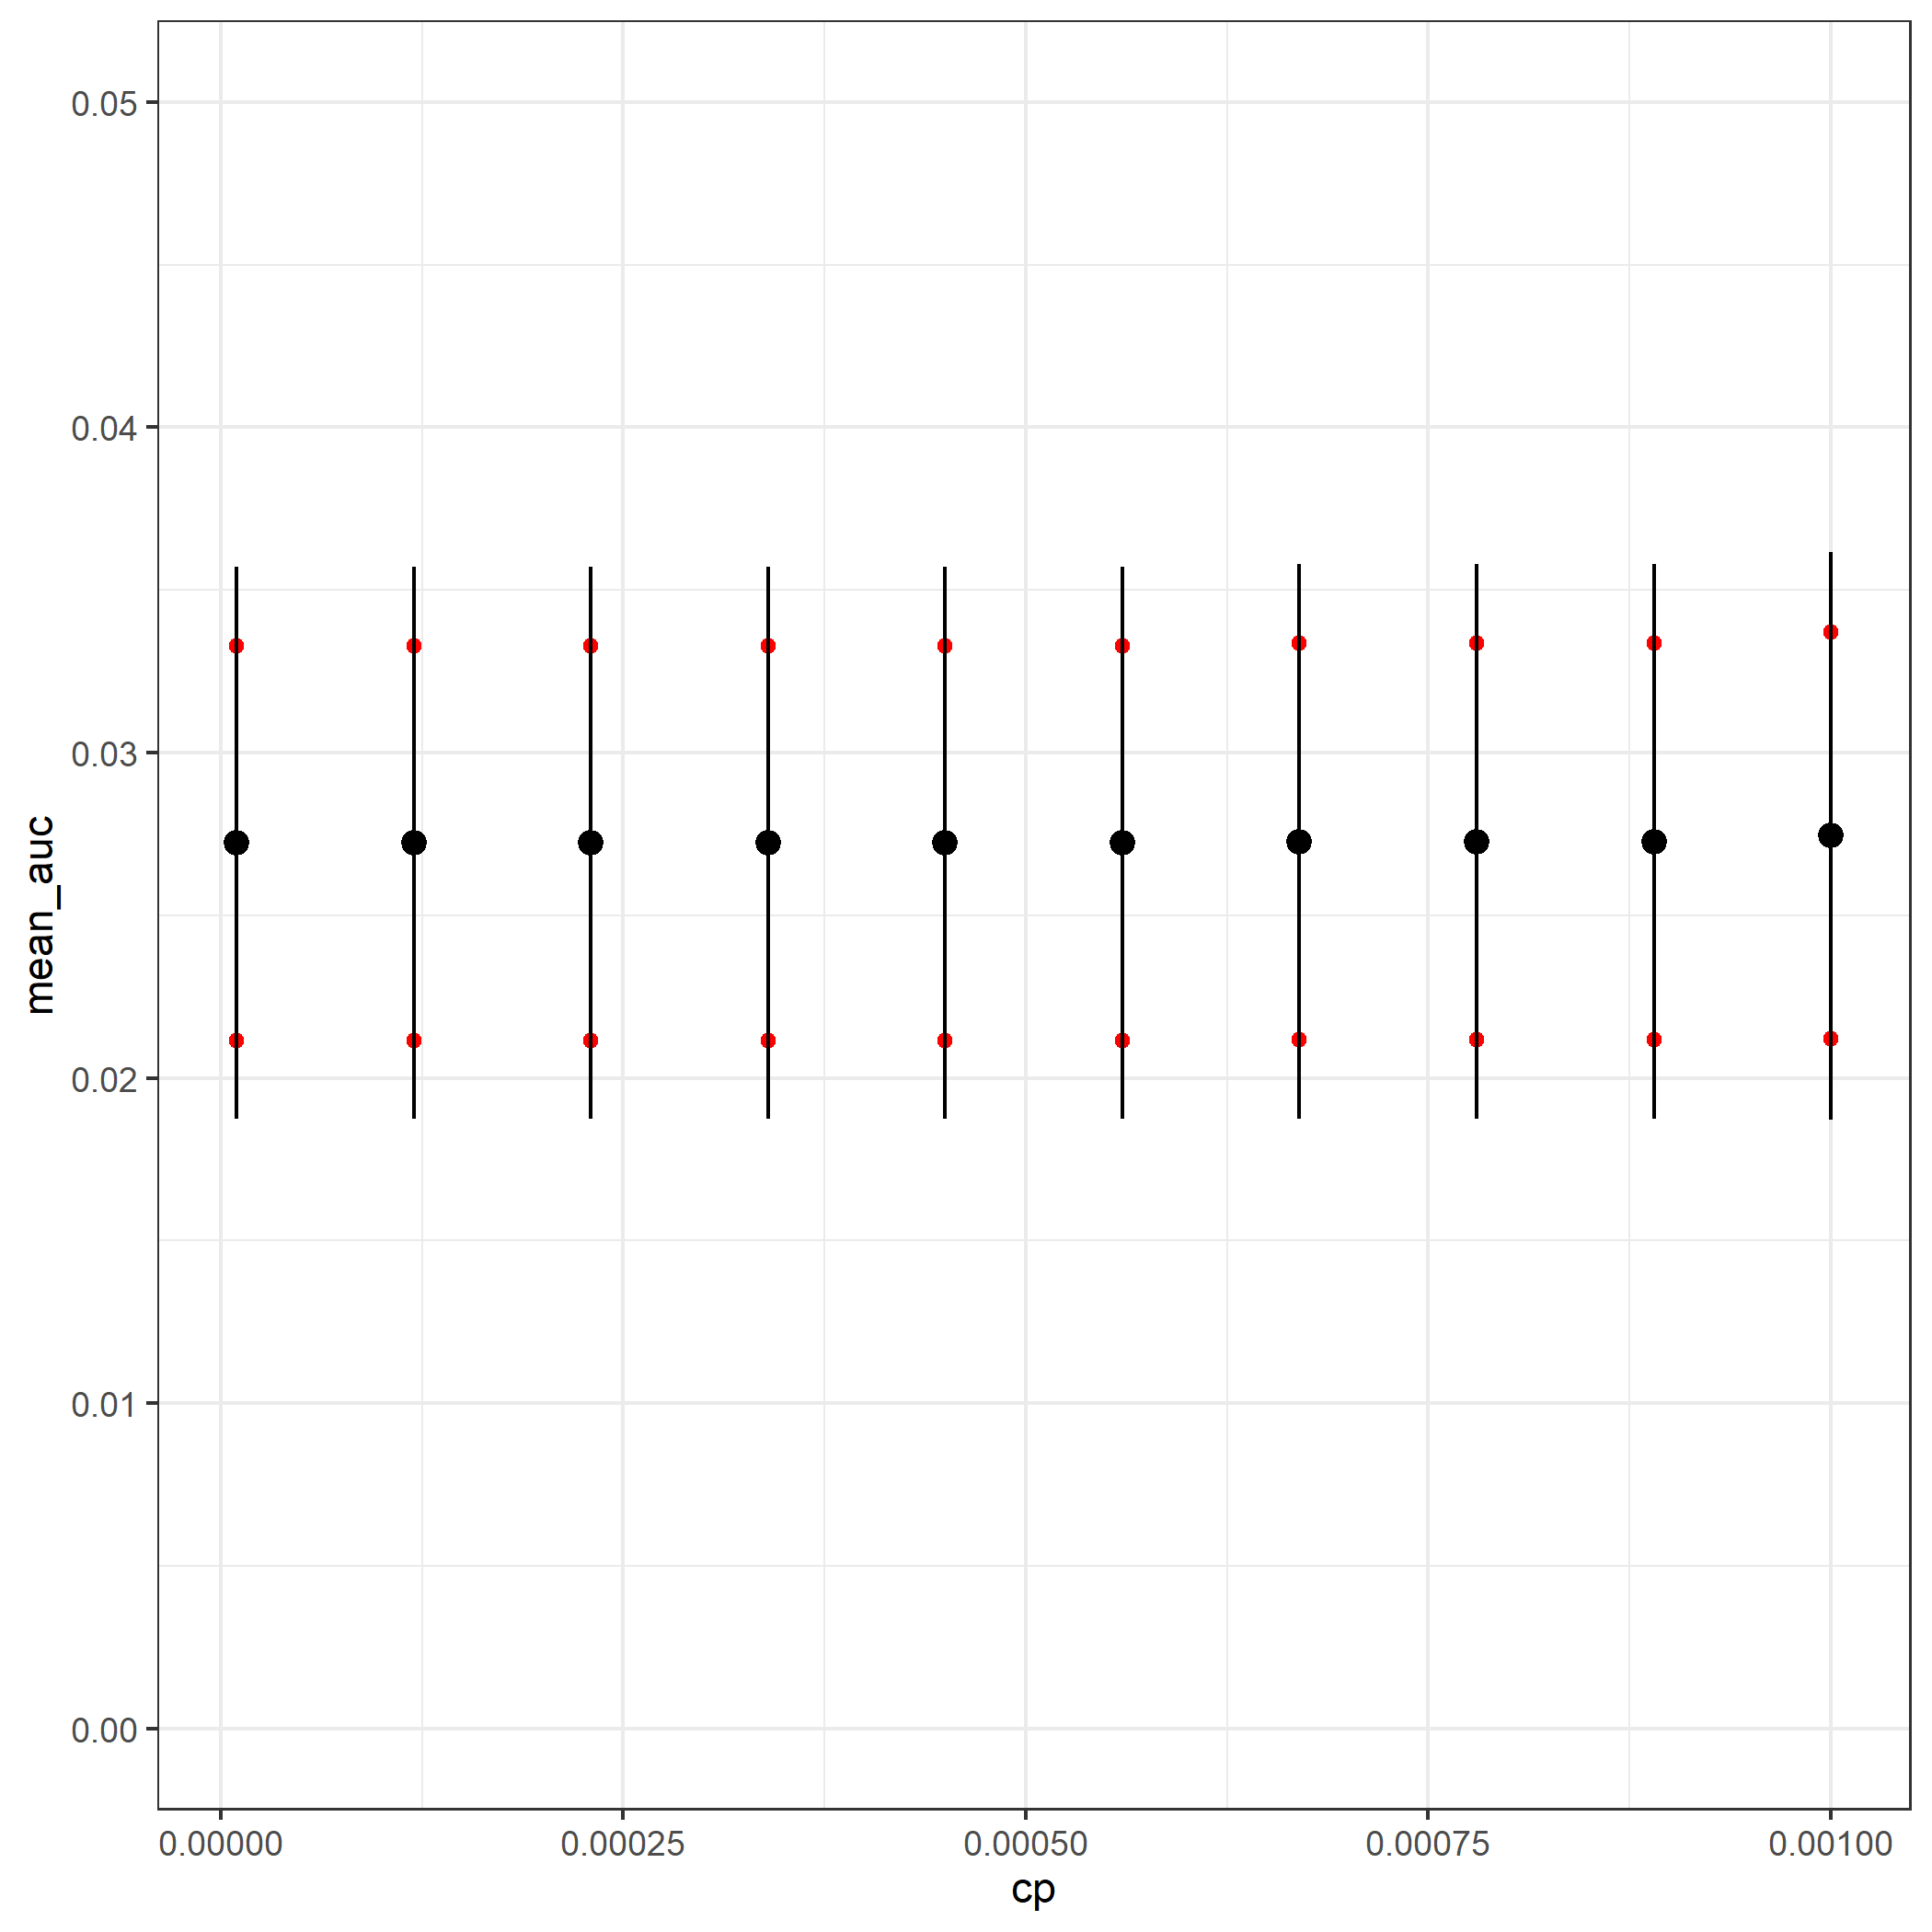
\includegraphics[width=30.15in]{data/cv_dt}

The graphique above shows the mean AUC as a function of different values of cp.~The black lines represent the standard deviation and the red dots the Confidence Intervals (computed with the \texttt{t.test()} function and with \(\alpha = 5\%\)).
As we can see the mean \(AUC_{0.2}\) stay stable for the six firsts values of \(cp\) and increase a bit for \(cp = 6.7\times10^{-3}\) and then stay stable with increasing \(cp\). Reducing the complexity parameter below \(cp = 0.001\) doesn't change the mean \(AUC_{0.2}\). The \(cp\) parameter indicates the minimum change of the training error rate to consider the splitting process. As a low \(cp\) means a more complex model, we are looking for the highest value of cp maximizing the mean \(AUC_{0.2}\). We can see that \(cp = 0.001\) is already sufficiently low. Thus, we can select \(cp = 0.001\) to learn the decision tree.

\hypertarget{random-forest}{%
\section{Random Forest}\label{random-forest}}

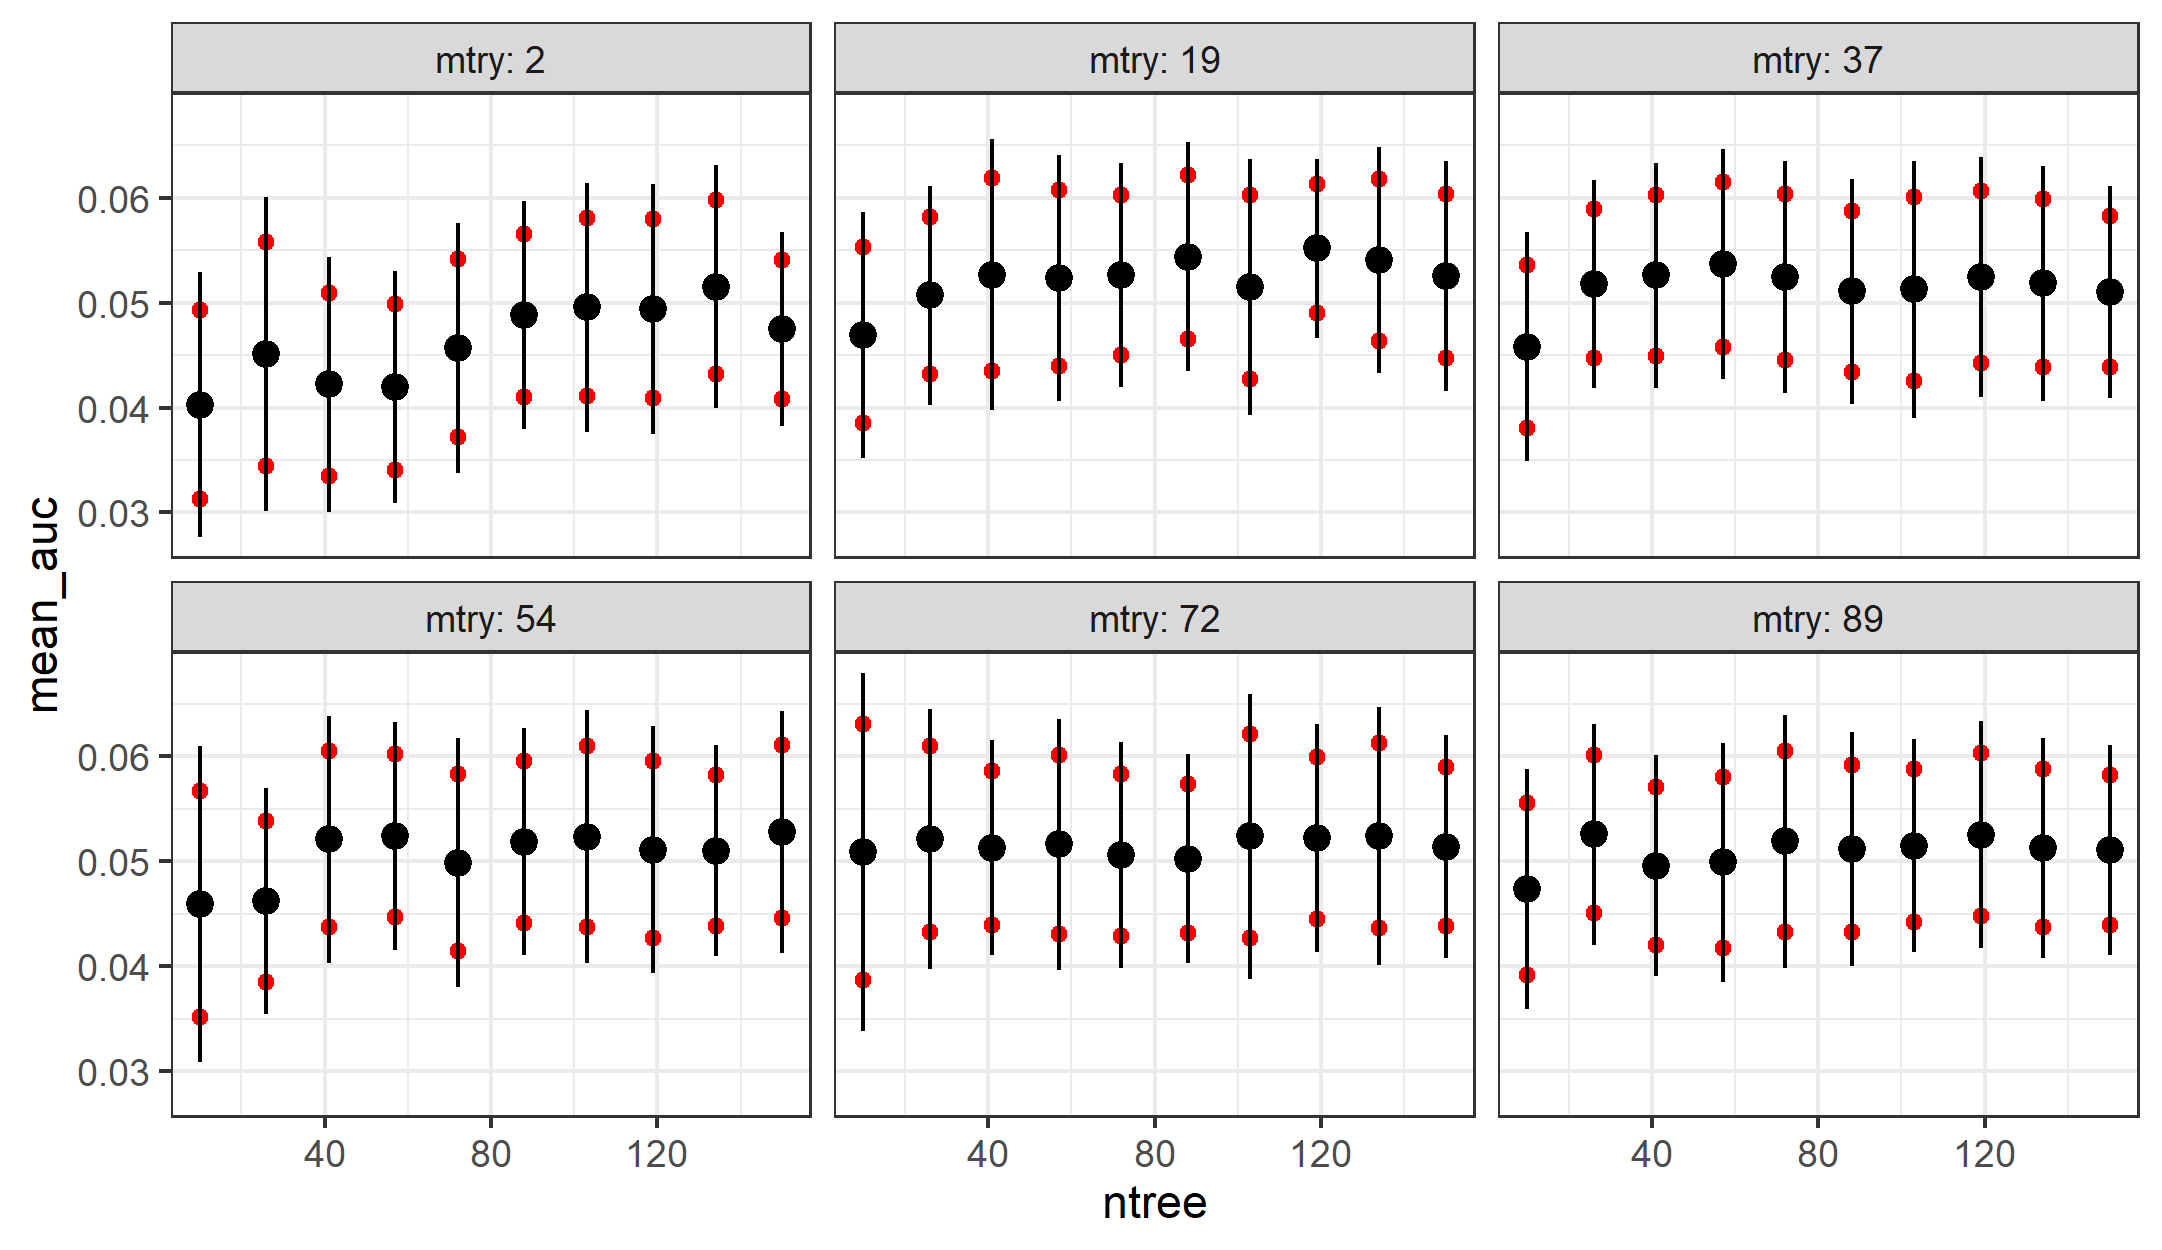
\includegraphics[width=30.03in]{data/cv_rf}

This plot shows the mean auc as a function of the number of trees (\emph{i.e.} \(ntree\)). Each square correspond to a value of \(mtry\), \emph{i.e.} the number of features used in the splitting process. As we can see, the highest value of \(AUC_{0.2}\) is for \(mtry = 19\) and \(ntree = 120\).

We know that the theoretical value of \(mtry\) for the classification task is \(\sqrt{number\:of\:feature}\). Here, it is equal to \(10\), which is quite close to the selected \(mtry = 19\).

\hypertarget{regularized-logistic-regression}{%
\section{Regularized logistic regression}\label{regularized-logistic-regression}}

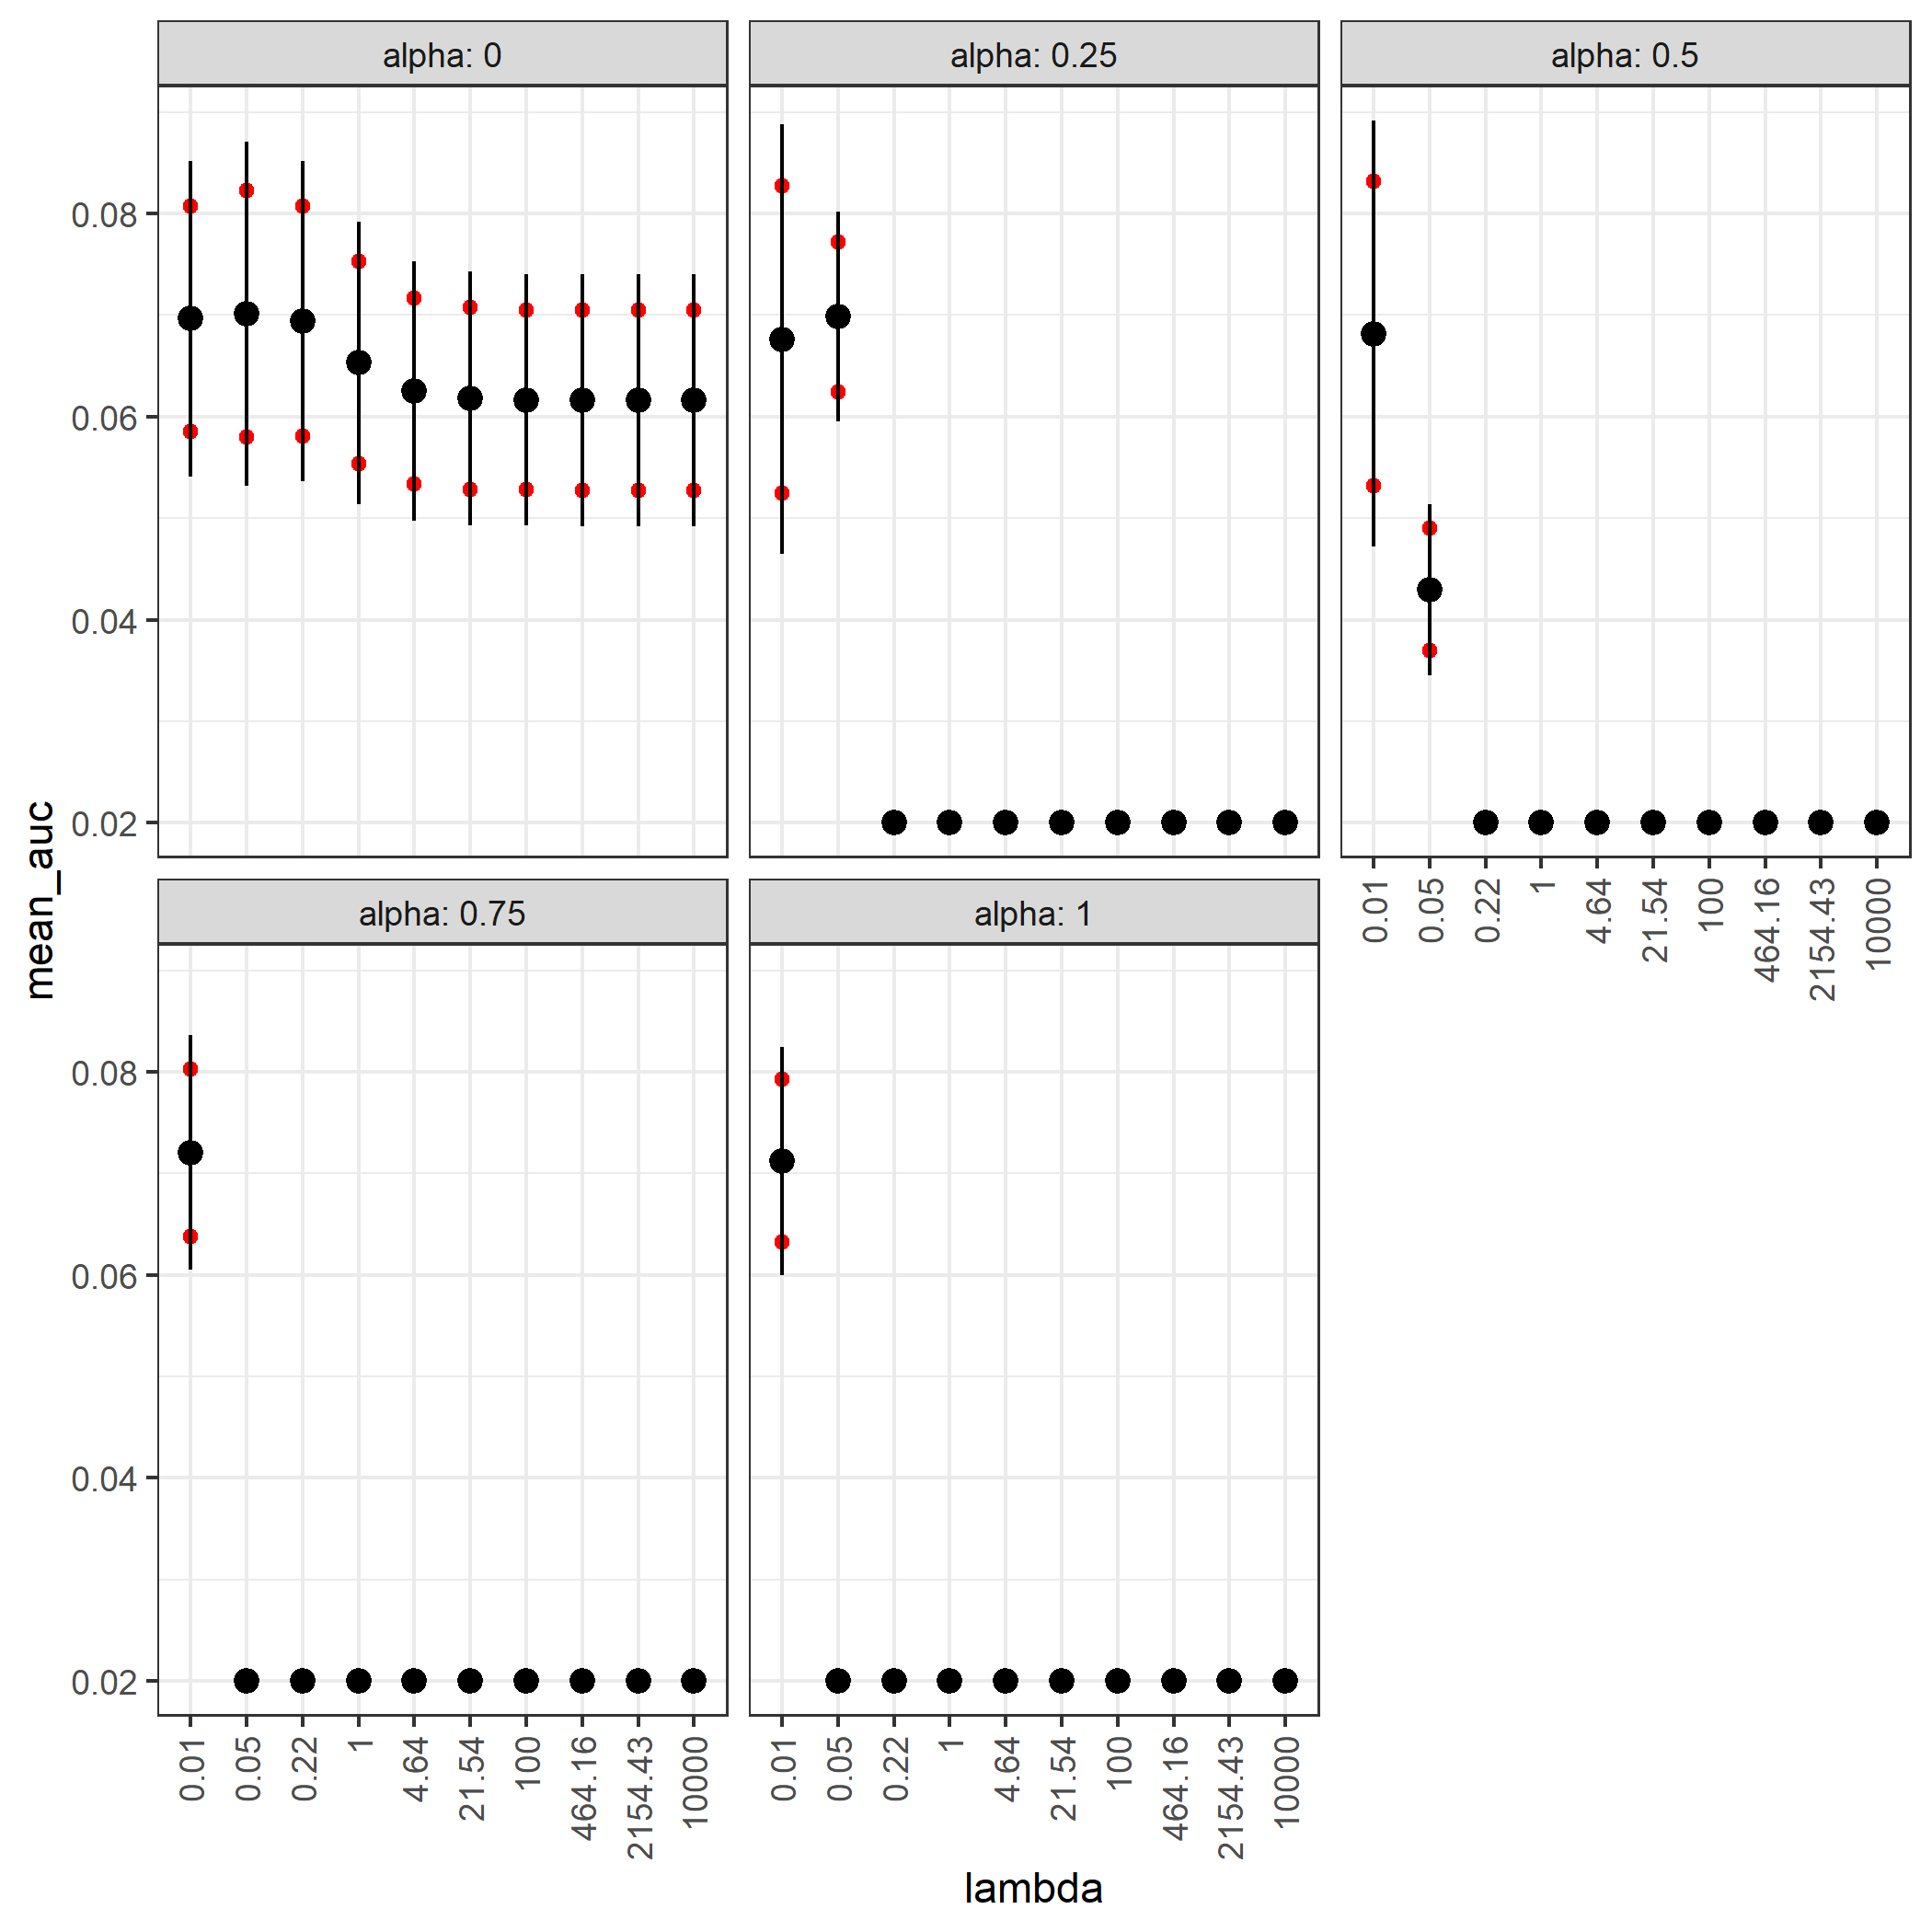
\includegraphics[width=29.17in]{data/cv_lr}

This figure shows the mean \(AUC_{0.2}\) for different values of two hyperparameters of the elastic net regularization:

\begin{itemize}
\item
  \(\alpha\): which is the weight given to the two types of penalties (L1 and L2, see \emph{Element of Statistical Learning}, Hastie \emph{et al.} 2001). \(\alpha = 1\) correspond to the lasso penalty (\emph{i.e.} the L1 penalty) and \(\alpha = 0\) correspont to the ridge regularization (\emph{i.e.} the L2 penalty).
\item
  \(\lambda\): which is the weighting of the penalties to the loss function. Thus, \(\lambda = 0\) means no weighting and is an unregularized logistic regression whilst \(\lambda = 1\) means a fully weighted penalty.
\end{itemize}

As we can see on this figures, the highest value of \(AUC_{0.2}\) seems to be for \(\alpha = 0.75\) and \(\lambda = 0.01\).

\hypertarget{note-about-hyperparameters-selection}{%
\section{Note about hyperparameters selection}\label{note-about-hyperparameters-selection}}

As represented on the previous plots, most of the \(AUC_{0.2}\) confidence intervals overlap, which means that their differences are statistically non significant. However, a choice was necessary and I decided to always choose the hyperparameters giving the lowest \(AUC_{0.2}\) values.

\hypertarget{evaluation-on-the-test-dataset}{%
\section{Evaluation on the test dataset}\label{evaluation-on-the-test-dataset}}

Thanks to the previous steps, we have chosen:

\begin{enumerate}
\def\labelenumi{\arabic{enumi}.}
\item
  Decision tree with \(cp = 0.001\)
\item
  Random forest with \(ntree = 120\) and \(mtry = 19\)
\item
  Regularized logistic regression with \(\lambda = 0.01\) and \(\alpha = 0.75\)
\end{enumerate}

Now, we can \textbf{1)} learn the model on the entire training dataset and \textbf{2)} compute the \(AUC_{0.2}\) when predicting on the test dataset.

The following plots show the ROC curve (Receiver Operating Characteristic) of the three optimized models with their respective \(AUC_{0.2}\) displayed in the table.

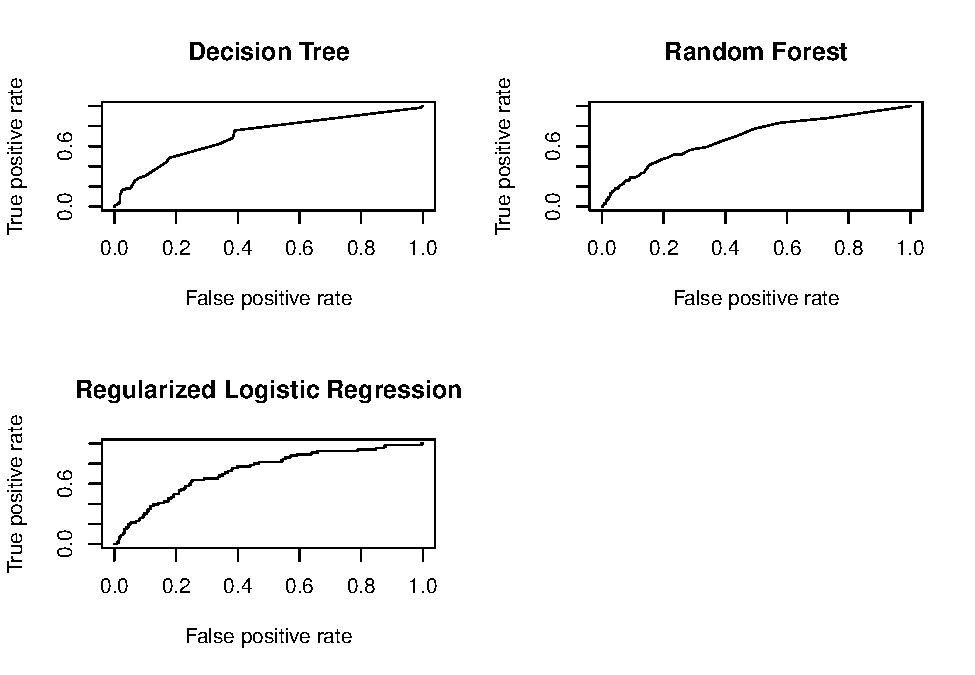
\includegraphics[width=1.5\linewidth]{leroy_francois_hw2_files/figure-latex/unnamed-chunk-17-1}

\begin{table}[H]
\centering
\begin{tabular}{l|r}
\hline
model & auc\\
\hline
Decision Tree & 0.060\\
\hline
Random Forest & 0.055\\
\hline
Regularized Logistic Regression & 0.056\\
\hline
\end{tabular}
\end{table}

As we can see, the highest value of \(AUC_{0.2}\) is for the decision tree with \(cp = 0.001\). It is interesting to note the difference between the \(AUC_{0.2}\) computed on the test dataset and the one computed from the cross-validation. From the cross-validation, the highest value of \(AUC_{0.2}\) was for the regularized logistic regression, with \(AUC_{0.2}\approx0.07\) whilst for the decision tree it was slightly lower than \(0.065\). Now, we can see that \(AUC_{0.2}\) is higher for the decision tree. We can think that the decision tree is better at generalization than the regularized logistic regression, which was slightly overfitted.

\hypertarget{setting-cutoff-threshold}{%
\section{Setting cutoff threshold}\label{setting-cutoff-threshold}}

The cut-off indicates the probability at which we should start to consider the prediction as True. The following plot shows the values of precision, accuracy, True Positive Rate (TPR) and False Positive Rate (FPR) according to different cut-off threshold. So far, all the learning processes have been done using the \(AUC_{0.2}\), which is the Area Under the Curve just up to \(FPR\leq20\%\). Thus, I decided not to consider cut-off higher than 0.2.

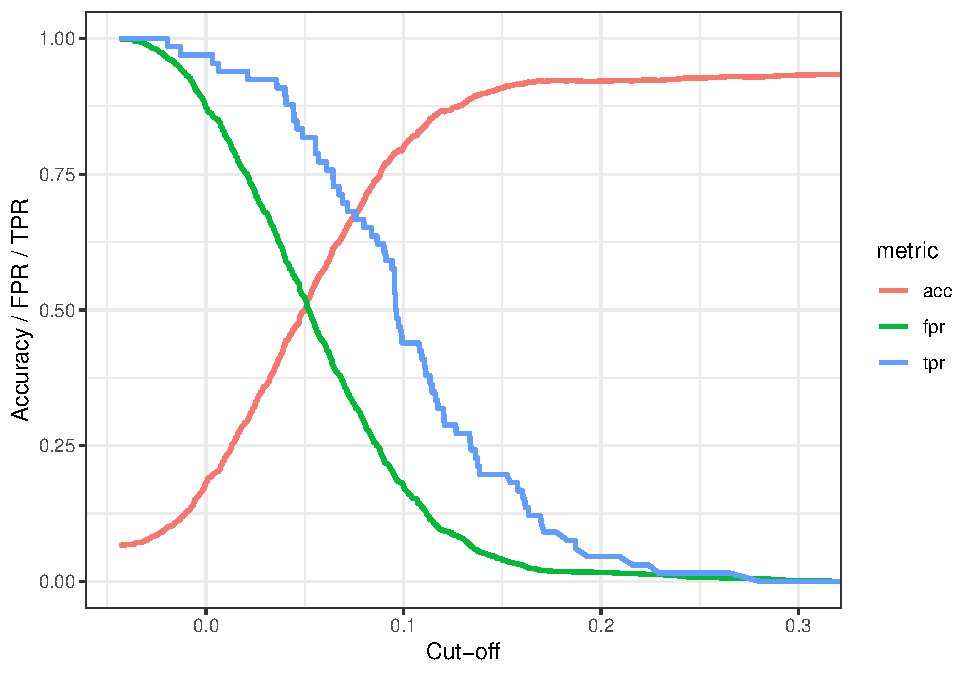
\includegraphics{leroy_francois_hw2_files/figure-latex/unnamed-chunk-19-1.pdf}

First, we can see that the precision and accuracy start closely to what a random classifier would do, \emph{i.e.} close to \(0.06\). We can also observe that the maximum value of accuracy is very quickly reach: this is due to the fact that our dataset is really homogeneous, \emph{i.e.} we have a lot of \emph{No} for very little \emph{Yes}. Thus, the classifier will quickly correctly classify all the actual \emph{No} as \emph{No} for low values of the cut-off and the accuracy will be high. Here, we need to focus on the correctly classified \emph{Yes}, and for this we use the precision (\(P = \frac{TP}{TP+FP}\)). We can see that the highest value of precision is reached for \(cutoff = 0.2\).

Now, we can compute the confusion matrix with a threshold of \(0.2\):

\begin{verbatim}
##     obs
## pred   0   1
##    0 894  54
##    1  40  12
\end{verbatim}

\hypertarget{task-3---model-interpretation-and-feature-selection}{%
\chapter{Task 3 - Model interpretation and feature selection}\label{task-3---model-interpretation-and-feature-selection}}

\begin{table}[H]
\caption{\label{tab:DT}Variable importance for the decision tree}

\centering
\fontsize{9}{11}\selectfont
\begin{tabular}[t]{l|r}
\hline
feature & MeanDecreaseGini\\
\hline
PPERSAUT & 16.39\\
\hline
PBRAND & 12.61\\
\hline
APERSAUT & 12.06\\
\hline
MKOOPKLA & 10.73\\
\hline
PWAPART & 9.52\\
\hline
MOSTYPE & 9.41\\
\hline
MFGEKIND & 9.25\\
\hline
MBERHOOG & 8.81\\
\hline
AWAPART & 8.71\\
\hline
MOSHOOFD & 7.16\\
\hline
MOPLMIDD & 6.77\\
\hline
MOPLLAAG & 6.68\\
\hline
MRELGE & 6.64\\
\hline
ABRAND & 6.16\\
\hline
MFWEKIND & 5.93\\
\hline
MINK4575 & 5.69\\
\hline
MGODGE & 5.58\\
\hline
MRELOV & 5.25\\
\hline
MZPART & 4.99\\
\hline
MOPLHOOG & 4.83\\
\hline
MZFONDS & 4.68\\
\hline
MBERARBG & 4.66\\
\hline
MSKA & 4.65\\
\hline
MGEMLEEF & 4.55\\
\hline
MHHUUR & 4.53\\
\hline
MSKB1 & 4.24\\
\hline
MINK3045 & 4.14\\
\hline
MGEMOMV & 3.85\\
\hline
\end{tabular}
\centering
\begin{tabular}[t]{l|r}
\hline
feature & MeanDecreaseGini\\
\hline
MBERMIDD & 3.81\\
\hline
MGODPR & 3.63\\
\hline
MINKGEM & 3.53\\
\hline
APLEZIER & 3.19\\
\hline
PPLEZIER & 3.19\\
\hline
MHKOOP & 3.14\\
\hline
MSKD & 3.12\\
\hline
MFALLEEN & 3.03\\
\hline
MSKC & 2.90\\
\hline
MGODOV & 2.85\\
\hline
MAUT0 & 2.73\\
\hline
MSKB2 & 2.63\\
\hline
MBERARBO & 2.52\\
\hline
MINK7512 & 2.35\\
\hline
MAUT1 & 2.10\\
\hline
MINKM30 & 1.83\\
\hline
MAUT2 & 1.77\\
\hline
MRELSA & 1.13\\
\hline
MAANTHUI & 0.83\\
\hline
MBERZELF & 0.79\\
\hline
MGODRK & 0.78\\
\hline
ALEVEN & 0.70\\
\hline
PLEVEN & 0.70\\
\hline
AWALAND & 0.34\\
\hline
PWALAND & 0.34\\
\hline
ABYSTAND & 0.31\\
\hline
PBYSTAND & 0.31\\
\hline
PTRACTOR & 0.30\\
\hline
\end{tabular}
\end{table}

The previous table \ref{tab:DT} shows the features ordered by decreasing value of the mean decrease of the Gini index for the deicision tree. The Gini index is an index of impurity. Low values of Gini indicate a purer leaf node. Thus, a higher decrease in the Gini index means a feature which is more prone to classify correctly.

\begin{table}[H]
\caption{\label{tab:RF}Variable importance for the random forest}

\centering
\fontsize{9}{11}\selectfont
\begin{tabular}[t]{l|r}
\hline
feature & MeanDecreaseGini\\
\hline
PBRAND & 20.09\\
\hline
MOSTYPE & 17.20\\
\hline
PPERSAUT & 16.73\\
\hline
APERSAUT & 14.74\\
\hline
MKOOPKLA & 11.94\\
\hline
PWAPART & 11.54\\
\hline
MGODGE & 11.08\\
\hline
MBERMIDD & 11.03\\
\hline
MGODPR & 10.97\\
\hline
MOPLMIDD & 10.90\\
\hline
MOSHOOFD & 10.27\\
\hline
MBERARBG & 10.12\\
\hline
MINK3045 & 9.88\\
\hline
MOPLLAAG & 9.86\\
\hline
MFGEKIND & 9.49\\
\hline
MFWEKIND & 9.46\\
\hline
MOPLHOOG & 9.39\\
\hline
MBERARBO & 9.11\\
\hline
MHHUUR & 8.98\\
\hline
MINK4575 & 8.82\\
\hline
MSKB1 & 8.74\\
\hline
MBERHOOG & 8.71\\
\hline
MSKC & 8.31\\
\hline
MHKOOP & 8.27\\
\hline
MINKGEM & 7.92\\
\hline
ABRAND & 7.72\\
\hline
MSKB2 & 7.66\\
\hline
AWAPART & 7.65\\
\hline
\end{tabular}
\centering
\begin{tabular}[t]{l|r}
\hline
feature & MeanDecreaseGini\\
\hline
MINKM30 & 7.55\\
\hline
MSKA & 7.47\\
\hline
MINK7512 & 7.41\\
\hline
MZFONDS & 7.40\\
\hline
MGODOV & 7.33\\
\hline
MFALLEEN & 7.29\\
\hline
MRELGE & 7.20\\
\hline
MAUT1 & 6.95\\
\hline
MZPART & 6.82\\
\hline
MRELOV & 6.26\\
\hline
MAUT0 & 6.18\\
\hline
MAUT2 & 5.99\\
\hline
MGEMLEEF & 5.83\\
\hline
ALEVEN & 5.55\\
\hline
MSKD & 5.39\\
\hline
PLEVEN & 5.07\\
\hline
MGEMOMV & 4.77\\
\hline
MGODRK & 4.72\\
\hline
AFIETS & 4.71\\
\hline
MRELSA & 4.61\\
\hline
MBERZELF & 4.37\\
\hline
PBYSTAND & 3.99\\
\hline
ABYSTAND & 3.73\\
\hline
PPLEZIER & 3.70\\
\hline
APLEZIER & 3.53\\
\hline
MBERBOER & 3.38\\
\hline
PMOTSCO & 3.24\\
\hline
MINK123M & 2.76\\
\hline
\end{tabular}
\centering
\begin{tabular}[t]{l|r}
\hline
feature & MeanDecreaseGini\\
\hline
AMOTSCO & 2.73\\
\hline
PBROM & 2.70\\
\hline
PFIETS & 2.62\\
\hline
ABROM & 2.44\\
\hline
MAANTHUI & 2.43\\
\hline
PWAOREG & 2.36\\
\hline
PGEZONG & 1.65\\
\hline
AWAOREG & 1.59\\
\hline
PTRACTOR & 1.20\\
\hline
PINBOED & 1.15\\
\hline
AGEZONG & 1.11\\
\hline
AINBOED & 1.02\\
\hline
PAANHANG & 0.97\\
\hline
PWABEDR & 0.88\\
\hline
ATRACTOR & 0.78\\
\hline
AWABEDR & 0.73\\
\hline
AAANHANG & 0.69\\
\hline
PBESAUT & 0.49\\
\hline
ABESAUT & 0.47\\
\hline
AZEILPL & 0.27\\
\hline
APERSONG & 0.25\\
\hline
PZEILPL & 0.22\\
\hline
AWALAND & 0.19\\
\hline
PPERSONG & 0.17\\
\hline
PWALAND & 0.15\\
\hline
PWERKT & 0.04\\
\hline
PVRAAUT & 0.01\\
\hline
AWERKT & 0.01\\
\hline
AVRAAUT & 0.00\\
\hline
\end{tabular}
\end{table}

The table \ref{tab:RF} also shows the mean decrease of the Gini index for each feature for the random forest.

\textbf{Feature analysis of the decision tree and the random forest:} we can observe from the decision tree (DT) and the random forest (RF) that the features \emph{PBRAND}, \emph{PPERSAUT}, \emph{APERSAUT} and \emph{PWAPART}, which correspond respectively to \emph{contribution fire policies}, \emph{contribution car policies}, \emph{number of car policies} and \emph{contribution private third party insurance}, seem to be important in classify the target values. Those previous features correspond to purchasing habits of customers. We can assume that the customers that are used to subscribe to policies are more likely to buy an insurance.

The second class of driving features are related to the socio-economic status of the customers. As expected, the \emph{MOSTYPE} and \emph{MOSHOOFD} features are determinant in the final purchase (see Task \ref{task1}). However, a new important feature appears in this tables: the \emph{MKOOPKLA} feature, which correspond to the \emph{purchasing power class} of the customers. We can expect that the higher the power class, the higher are the chance of purchasing an insurance policy. This assumption is validated by the output of the lasso logistic regression (table \ref{tab:lasso}) where we can see the positive value of the coefficient for the \emph{MKOOPKLA} feature.

\begin{table}[H]
\caption{\label{tab:lasso}Variable importance for the lasso regression}

\centering
\fontsize{9}{11}\selectfont
\begin{tabular}[t]{l|r}
\hline
feature & s0\\
\hline
APLEZIER & 1.2945711\\
\hline
AZEILPL & 1.1414119\\
\hline
ABYSTAND & 0.7523564\\
\hline
AFIETS & 0.4165938\\
\hline
PWAOREG & 0.2678450\\
\hline
PPERSAUT & 0.2038757\\
\hline
MBERBOER & -0.1672857\\
\hline
PWAPART & 0.1551758\\
\hline
MINK123M & -0.1506243\\
\hline
PWALAND & -0.1470406\\
\hline
ATRACTOR & -0.1432662\\
\hline
PBRAND & 0.1026457\\
\hline
MINKGEM & 0.0765117\\
\hline
MRELGE & 0.0675735\\
\hline
MOPLLAAG & -0.0633978\\
\hline
\end{tabular}
\centering
\begin{tabular}[t]{l|r}
\hline
feature & s0\\
\hline
PWABEDR & -0.0584269\\
\hline
MOPLHOOG & 0.0515774\\
\hline
MGODRK & -0.0435352\\
\hline
MAUT1 & 0.0356634\\
\hline
MHHUUR & -0.0344877\\
\hline
MBERMIDD & 0.0309560\\
\hline
PGEZONG & 0.0288318\\
\hline
MGEMLEEF & 0.0271291\\
\hline
PWERKT & -0.0263719\\
\hline
MGODGE & -0.0245771\\
\hline
PBESAUT & -0.0218699\\
\hline
MKOOPKLA & 0.0191547\\
\hline
MRELSA & -0.0169228\\
\hline
MINK7512 & 0.0124976\\
\hline
MSKD & -0.0099615\\
\hline
PLEVEN & -0.0020227\\
\hline
\end{tabular}
\end{table}

This last table \ref{tab:lasso} shows the features selected by the lasso regularization. I decided to display only the feature for which the coefficients are different from zero. In this table, the coefficient can be interpreted as for a logistic regression: the value of the coefficient describe the variation of the log odds for a unit change of this feature.

\textbf{Interpretation of the features selected by the lasso regression and comparisons with the DT and the RF:} surprisingly, we can see that the features selected are quite different from the ones by the DT and the RF. One can think that the lasso regression, by taking off some features, also takes off the co-interactions of several features on the target attribute. Thus, features that were driving the classification by interacting with other features are reconsidered. One can think that the lasso regression allows to see the actual/true impact of the features on the target attributes.

Interestingly, the \emph{MOSTYPE} and \emph{MOSHOOFD} features don't appear in the lasso regularization. However, the \emph{MKOOPKLA} is selected, with the positive impact expected. Here, the four firsts features each correspond to the number of different insurances of the customers, with all a positive coefficients. It means that the more numerous insurance a customer have, the more likely he will subscribe to an insurance. It is important to note that the \emph{MBERBOER} (\emph{i.e.} the farmers) feature has a negative impact, which means that the farmers are less likely to buy an insurance. One last important and surprising thing to note is the negative impact of the \emph{MINK123M} feature, which correspond to \emph{Income \textgreater123.000}. This results means that customers with a high income are less likely to subscribe an insurance policy. First, this is not expected and second, it goes against the positive relationship with the \emph{MINKGEM} feature, which is the \emph{average income} and which means that wealthier customers are more prone to subscribe to an insurance policy.

\hypertarget{task-4---final-prediction-on-the-blind-test-set}{%
\chapter{Task 4 - Final prediction on the blind test set}\label{task-4---final-prediction-on-the-blind-test-set}}

The final prediction is done using the Decision Tree with a complexity parameter of \(0.001\) chosen because of its highest \(AUC_{0.2}\). However, when setting the cut-off threshold to \(0.2\), I noticed that the number of 1 are slightly lower than 100. Thus, I decided to take the 100 firsts highest probabilities of \(P(\hat{y} = 1)\) and make them equal to 1.

\begin{Shaded}
\begin{Highlighting}[]
\KeywordTok{set.seed}\NormalTok{(}\DecValTok{123}\NormalTok{)}
\CommentTok{## Load the blind dataset}
\NormalTok{T <-}\StringTok{ }\KeywordTok{read.delim}\NormalTok{(}\StringTok{"data/test_data_t.csv"}\NormalTok{,}
                \DataTypeTok{header=}\OtherTok{FALSE}\NormalTok{)}
\CommentTok{## Write the column names}
\KeywordTok{colnames}\NormalTok{(T) <-}\StringTok{ }\KeywordTok{colnames}\NormalTok{(d_train)[}\OperatorTok{-}\DecValTok{86}\NormalTok{]}
\CommentTok{## Predict}
\NormalTok{final_pred <-}\StringTok{ }\KeywordTok{predict}\NormalTok{(opti_DT, T, }\DataTypeTok{type =} \StringTok{"prob"}\NormalTok{)[,}\DecValTok{2}\NormalTok{]}
\CommentTok{## Convert the 100 firsts highest proba to 1 and the 900 others to 0}
\NormalTok{final_pred <-}\StringTok{ }\NormalTok{final_pred }\OperatorTok\StringTok{ }\KeywordTok{as_tibble}\NormalTok{() }\OperatorTok\StringTok{ }
\StringTok{  }\KeywordTok{mutate}\NormalTok{(}\DataTypeTok{id =} \KeywordTok{seq}\NormalTok{(}\KeywordTok{nrow}\NormalTok{(.))) }\OperatorTok\StringTok{ }\KeywordTok{arrange}\NormalTok{(}\KeywordTok{desc}\NormalTok{(value))}
\NormalTok{final_pred[}\DecValTok{1}\OperatorTok{:}\DecValTok{100}\NormalTok{, }\DecValTok{1}\NormalTok{] <-}\StringTok{ }\DecValTok{1}
\NormalTok{final_pred[}\DecValTok{101}\OperatorTok{:}\KeywordTok{nrow}\NormalTok{(final_pred), }\DecValTok{1}\NormalTok{] <-}\StringTok{ }\DecValTok{0}
\NormalTok{final_pred <-}\StringTok{ }\NormalTok{final_pred }\OperatorTok\StringTok{ }\KeywordTok{arrange}\NormalTok{(id) }\OperatorTok\StringTok{ }\KeywordTok{pull}\NormalTok{(value)}
\CommentTok{## Check that n(1)=100 and n(0)=900}
\KeywordTok{table}\NormalTok{(final_pred)}
\end{Highlighting}
\end{Shaded}

\begin{verbatim}
## final_pred
##   0   1 
## 900 100
\end{verbatim}

\begin{Shaded}
\begin{Highlighting}[]
\CommentTok{## Save it}
\KeywordTok{write}\NormalTok{(final_pred, }\StringTok{"data/T.prediction.txt"}\NormalTok{, }\DataTypeTok{ncolumns =} \DecValTok{1}\NormalTok{)}
\end{Highlighting}
\end{Shaded}


\singlespacing % reset the spacing of the bibliography style
\end{document}
